\chapter{INTRODUCTION TO THE STANDARD MODEL}\label{Ch1}

The Particle Physics is probing the smallest objects that are known as elementary particles and tries to extend our knowledge of the subatomic world. These elementary particles are accelerated, collided and detected at very high energies in the experiments around the globe - one of them being the largest experimental setup ever built for science - and studied after being detected. The Standard Model of particle physics (SM) is the theory of the fundamental interactions in this pursuit. It is a quantum field theory developed with the contribution of many scientists around the globe mainly in the second half of the 20$^{th}$ century and, over the last few decades, it has been shown to be an accurate description of the picture. It describes all known particles but is a mathematical description of three of the four known fundamental forces of the nature. These are the electromagnetic interaction, the weak and the strong nuclear interactions. The gravitational force, due to difficulties in combining general relativity with quantum mechanics, does not take place in the Standard Model. The gravity is known to be 10$^{40}$ times weaker than the electromagnetic force, thus its effects are expected to be negligible in the theory.

In the SM, the elementary particles of matter and the ones that carry forces between them is grouped into two, namely fermions and bosons. The distinction shows itself in their spin properties; fermions have a spin value of half an integer whereas the bosons have integer spin values. Besides, the fermions obey the Pauli exclusion principle meaning that they cannot be at the same quantum state, whereas the bosons do not obey the same rule. The first generation of fermions include up and down quarks, electron and its neutrino pair; and bosons include photons, W and Z bosons, gluons and the Higgs boson. When added the second and the third generation of particles - whose existence is one of the mysteries of nature - along with their anti-particles, they form the fundamental particles that are known today. A tabular form of these particles can be seen in~\autoref{SM-figure}.

\vspace{6pt}
\begin{figure}[h]
	\centering
	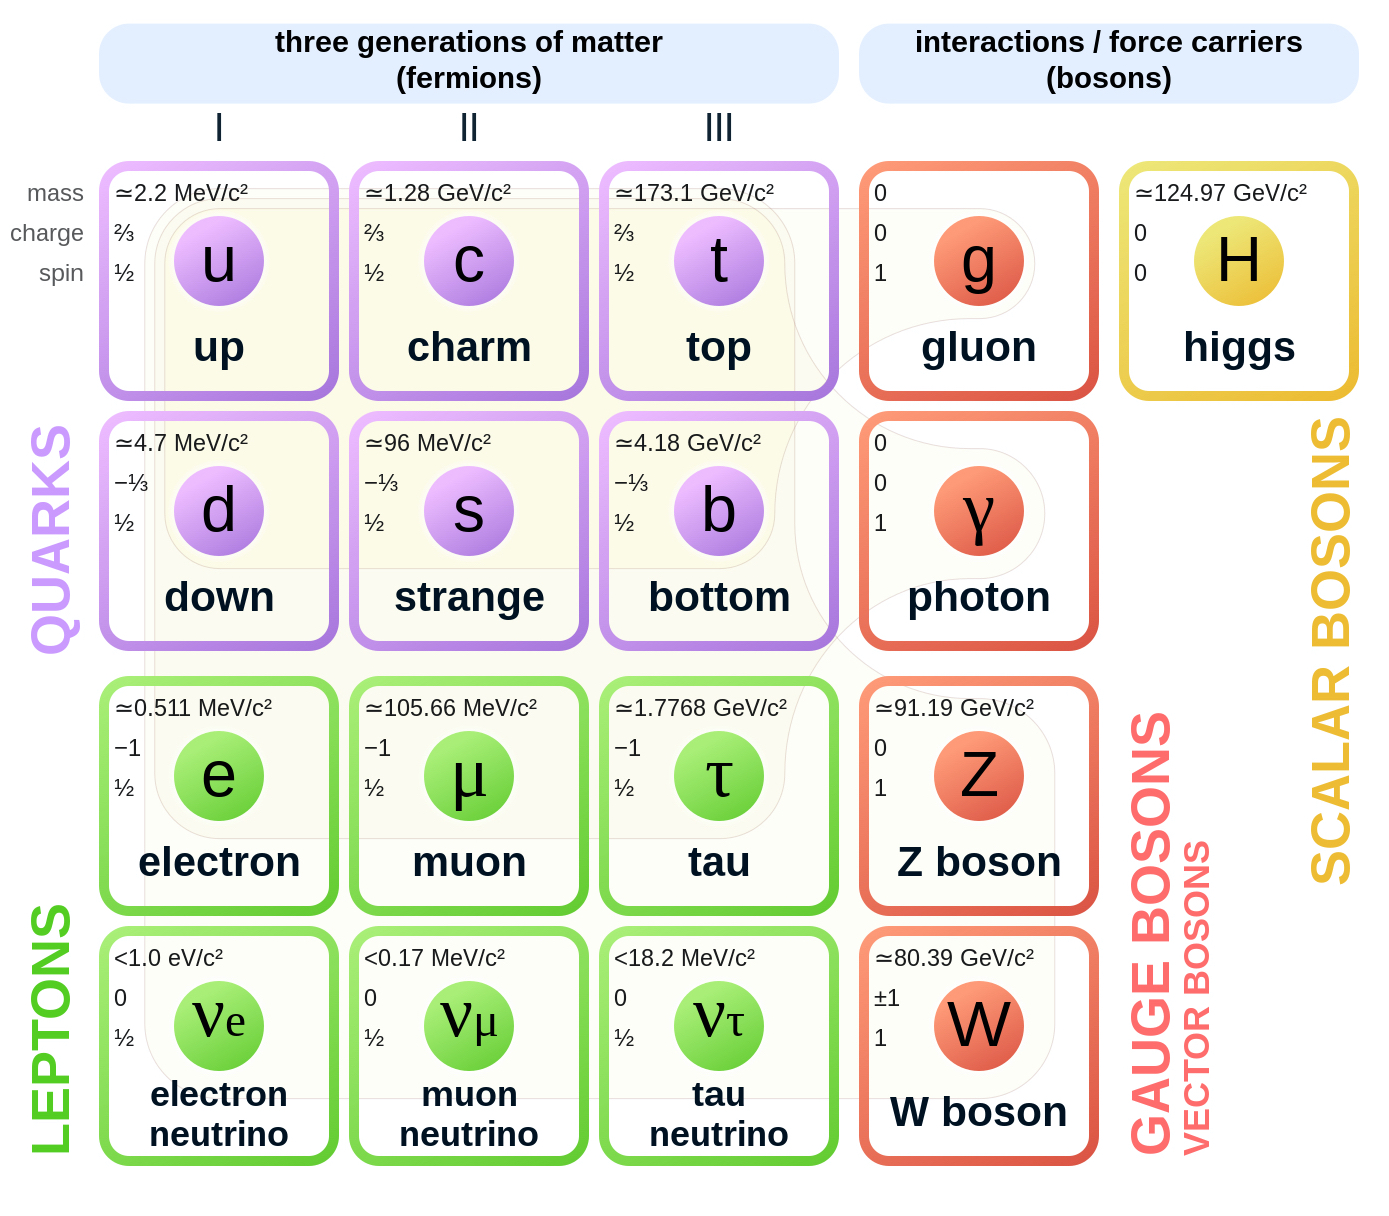
\includegraphics[width=\textwidth]{./SM.jpg}
	\vspace{6pt}
	\caption{The elementary particles of the Standard Model. The fermions and bosons are grouped in columns where the quarks, leptons, gauge bosons and scalar Higgs boson are shown in different colours. The three generations of matter are indicated with roman numerals. The mass, charge and spin values corresponding to each particle are indicated on the upper left of each box. The bosons are shown in faint yellow areas with which they interact with\cite{SM-ref}.}
	\label{SM-figure}
\end{figure}

Fermions make up the ordinary matter that we see around us everyday. A subgroup of fermions are the leptons and they include electron, muon, tau and their neutrino pairs. Neutrinos have very small mass values compared to other leptons and quarks. They do not have electromagnetic charge which makes them obey only the weak force and they barely interact with matter. Flavours of leptons other than the neutrinos (electrons, muons and taus) have sizeable mass and charge and they are members of the three generations of matter.

The other type of leptons are the quarks. They have three generation as leptons do, and they include six different flavours, namely up, down, charm, strange, top and bottom quarks. They interact with electromagnetic, weak and strong nuclear forces since they have colour charges in addition to their electric charge. 

Bosons are the mediator particles of the three forces described in the SM. The particles of this type are called the gauge boson and they include the photon ($\gamma$), W$^{\pm}$ bosons, Z boson, gluons and the Higgs boson. The photons and gluons do not have mass where W bosons have about 80 GeV/c$^{2}$, Z boson has 91 GeV/c$^{2}$ and the Higgs boson has 125 GeV/c$^{2}$ of mass. Among these, only the W$^{\pm}$ bosons have electric charge, and only the Higgs boson has a spin value of zero making it a scalar boson where all other bosons are spin-1 gauge bosons, meaning that they are vector bosons.

The electromagnetic force, whose quantum field theory is established by the \emph{Quantum Electrodynamics (QED)}, is mediated by photons and acts only on the charged particles.  Almost everything we see in the daily life is thanks to the electromagnetic interactions. The carrier of this force, the photons, do not have the charge of the interaction type, hence do not self-interact. Since the photons have zero mass, their interaction range is unlimited.

The weak interaction, which is responsible for the decay of the particles that is a flavour changing interaction, acts only on the fermions. It has a very short interaction range. The neutral and the charged current interactions are mediated by the vector bosons of the this force, the Z boson and the W$^{\pm}$ bosons, respectively. The Higgs boson in this picture, plays the role of generating the masses of the W$^{\pm}$, and Z bosons through the Higgs mechanism, and of the quarks and charged leptons through the Yukawa interaction.

\emph{Quantum Chromodynamics (QCD)} is the theory of the strong interaction and describes the interaction between quarks mediated by the massless gluons. It has an interaction range of about $10^{-15}$ m. Unlike the electromagnetic interaction, the gauge bosons of the strong force possess the charge of the interaction, namely colours, hence can couple to itself. There are 3 types of colour; red, green and blue. Each quark in the universe carry one of the 3 colours - they carry anti-colour if they are anti-quarks - and gluons can be thought of colour carrier particles. A phenomenon called the \emph{colour confinement} states that colour-charged particles cannot be isolated, meaning that only colour-neutral particles can be observed in nature\footnotemark. This results in that gluons carry a pair of charge consisting a colour and an anti-colour. Also, the hadrons are colour-neutral in two ways; i) with a pair of colour and anti-colour ii) with 3 different types of colour or anti-colour. The first combination makes up mesons, consisting of a quark pair (a quark and an anti-quark) and the second combination forms baryons. 

\footnotetext{~Reference}

Electromagnetic and weak interactions are unified in a theory called the electroweak theory which is an $SU(2)_L \otimes U(1)_\gamma$ gauge group as described by the Brout-Englert-Higgs (BEH) mechanism. The SU(2)$_L$ and U(1)$_\gamma$ groups mix and give rise to the W$^{\pm}$, Z and $\gamma$ bosons.

\section{The Standard Model Lagrangian}\label{purposeofthesis}

Lorem ipsum dolor sit amet

\section{Fundamental Interactions}\label{literaturereview}

Lorem ipsum dolor sit amet

\subsection{The Higgs Boson}

Lorem ipsum dolor sit amet

\section{BSM Searches}

Lorem ipsum dolor sit amet
